\chapter{DNS Grid Independence Supplementary Diagnostics}
\label{app:dns_grid_indep_supp}

This appendix collects the per-field log-log convergence and the secondary time-series diagnostics for the four-grid DNS sweep summarised in \S\ref{subsec:dns_grid_indep} and Table~\ref{tab:dns_grid_indep}.

\begin{figure}[!htbp]
    \centering
    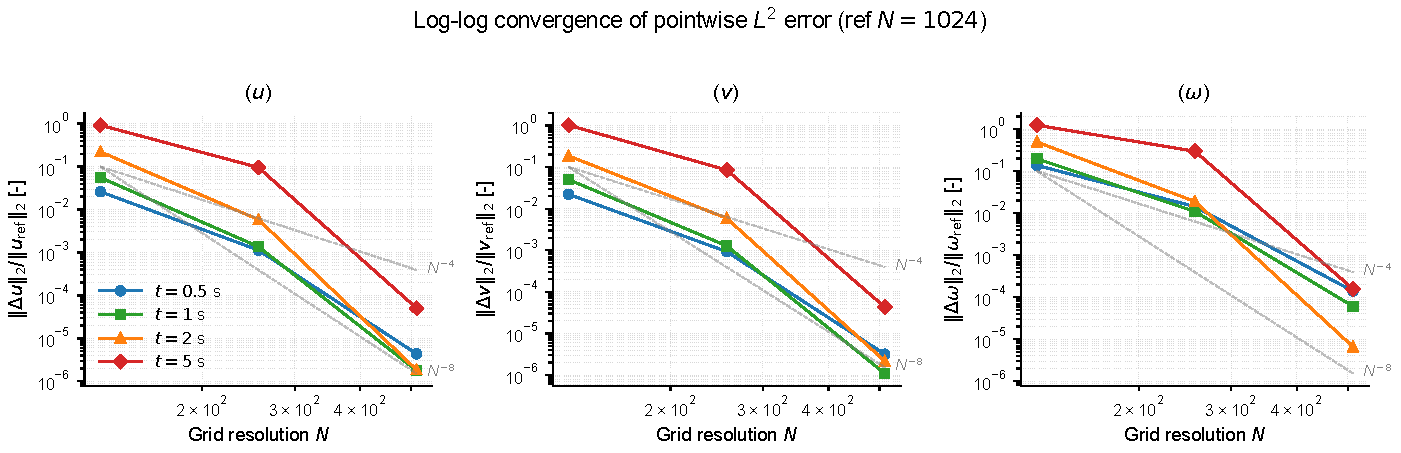
\includegraphics[width=\textwidth]{figures/results/grid_indep_supp_loglog.pdf}
    \caption{Log-log pointwise $L^2$ convergence against the $N=1024$ reference for the four-grid sweep at $Re=10^4$, evaluated at $t \in \{0.5, 1, 2, 5\}$~s. Each panel reports one field ($u$, $v$, $\omega$); dashed grey lines mark the algebraic reference slopes $N^{-4}$ and $N^{-8}$. Short-time slopes ($t \le 2$~s) lie steeper than $N^{-8}$, characteristic of pseudo-spectral super-algebraic convergence on a smooth IC; the $t=5$~s slope is shallower because pointwise error late in the chaotic trajectory is bounded by chaos amplification rather than discretisation truncation (statistical metrics in Fig.~\ref{fig:grid_indep_main}(a) remain at $0.064\%$).}
    \label{fig:grid_indep_supp_loglog}
\end{figure}

\begin{figure}[!htbp]
    \centering
    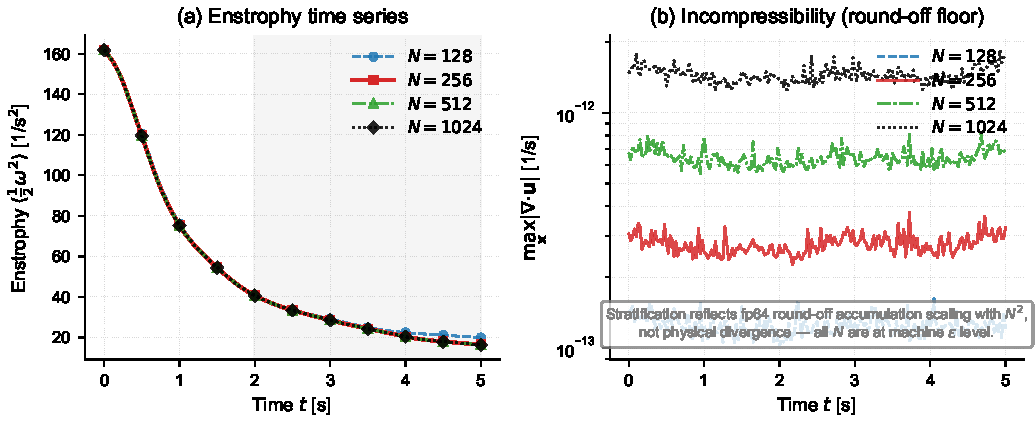
\includegraphics[width=\textwidth]{figures/results/grid_indep_supp_enstrophy_div.pdf}
    \caption{Secondary time-series diagnostics for the four-grid sweep. (a) Enstrophy $\langle \omega^2/2 \rangle(t)$; $N \ge 256$ overlap throughout, with the post-spin-up window ($t \ge 2$~s) shaded. (b) Maximum spectral incompressibility $\max_{\mathbf{x}} |\nabla \cdot \mathbf{u}|(t)$. All four grids sit at the fp64 round-off floor ($<10^{-11}$~1/s throughout); the apparent stratification reflects round-off accumulation scaling with $N^2$ over $\sim 10^5$ time steps rather than physical divergence.}
    \label{fig:grid_indep_supp_enstrophy_div}
\end{figure}

